\documentclass[11pt,article,oneside,a4paper]{abntex2}
\usepackage{graphicx}
\usepackage[portuguese,linesnumbered]{algorithm2e}
\usepackage[table]{xcolor}
\usepackage{multirow}
\usepackage{setspace}
\usepackage[labelfont={bf,small},textfont={bf,small},labelsep=endash]{caption}
\usepackage{filecontents}
\usepackage{verbatim}
\usepackage{mdwlist}
\usepackage{listings}
\usepackage{amsmath}
\usepackage[alf]{abntex2cite}
\usepackage{longtable}
\usepackage{lmodern}
\usepackage{afterpage}
\usepackage{pdflscape}
\usepackage{epstopdf}
\usepackage{indentfirst}
\usepackage{microtype}
\usepackage[utf8]{inputenc} 
\usepackage{subcaption}
\usepackage{mdwlist}
\usepackage{listings}

\begin{document}

\title{KDD em acidentes na cidade de Porto Alegre}
\author{Gustavo Jandt Feller, William Prigol Lopes}
\maketitle

\section{Introdução}

Através da aplicação de técnicas de KDD o presente trabalho vem apresentar os resultados de uma análise sobre os acidentes ocorridos na cidade de Porto Alegre de forma a recomendar alterações no trânsito da cidade para diminuir o número de acidentes, principalmente os acidentes do tipo fatais. 

Para tanto, abaixo temos a descrição dos objetivos do artigo (seção \ref{sec:objetivos}), a descrição do dataset (seção \ref{sec:dataset}), em seguida as análises inferidas sobre o dataset (seção \ref{sec:analise}) e conclusões acerca do dataset (seção \ref{sec:conclusao}).

\section{Contexto e justificativa do problema}

Os acidentes de trânsito envolvendo veículos, conforme as estatísticas indicam, é a forma de transporte ao qual mais mortes tem, mesmo em análises de percentuais de pessoas transportadas em relação a quantidade de mortes. Na cidade de Porto Alegre, a situação não é diferente. Com um planejamento urbano de décadas ao qual não se imaginava uma quantidade de carros tão grande quanto a atual, engarrafamentos e acidentes fazem parte do cotidiano da cidade, sendo que, devido a vários fatores, acidentes fatais naturalmente ocorrem.

Para isso, uma gestão que venha a tomar ações para evitar acidentes permitiria não só a diminuição de mortes mas um trânsito mais seguro, sendo assim, a decisão baseada em fatos virá a auxiliar no que fazer para diminuir os acidentes e, por meio dos processos de KDD, a identificação de fatores que venham de encontro com as necessidades de melhoria na cidade.

\section{Objetivos}
\label{sec:objetivos}

Para uma melhor interpretação das informações, dois tipos de objetivos são apresentados, os objetivos de negócio, contendo informações envolvidas com as decisões do gestor e objetivos de mineração envolvendo informações sobre a forma de tratamento dos dados.

Como \textbf{objetivo de negócio}, a ideia é posicionar-se visão de um gestor da área de trânsito publico, abordando o problema dos acidentes de trânsito na cidade de Porto Alegre. O principal objetivo do estudo é propor ações para mitigar os sinistros em situações nas quais ocorrem os acidentes.

Primeiramente interpretar um estudo geral do comportamento dos acidentes e dos locais dos acidentes e, em seguida, analisar fatores que envolvem os acidentes fatais. 

Assim, a aplicação de técnicas KDD nos \textit{datasets} públicos tem como objetivo encontrar informações que possam levar a tomada de decisões baseadas em fatos, criando suporte para concluir ações que possam ser tomadas pelo gestor para diminuir os acidentes na cidade de Porto Alegre.

Como \textbf{objetivo de mineração} tem-se a análise das variáveis do \textit{dataset} para compreender o comportamento dos acidentes, como histogramas, análises de correlação e clusterização. Também, um processo de densidade em latitude e longitude foi desenvolvido de forma a verificar os locais dos acidentes em uma forma mais visual.

A seguir, na seção \ref{sec:dataset} são apresentadas informações dos datasets envolvidos no presente trabalho.

\section{Dataset}
\label{sec:dataset}

Os \textit{datasets} utilizados para efetuar as análises\footnote{Disponível em www.datapoa.com.br/datasets} são três. O principal dataset contêm informações sobre os acidentes registrados na cidade de Porto Alegre compreendido um período de 14 anos (2000 a 2014). 

Contendo um total de 44 colunas, o \textit{dataset} apresenta uma quantidade de informações interessantes para análise devido a ter 14 anos de histórico. O descritivo das colunas do dataset é ilustrado na Tabela \ref{tab:dataset1}.

\begin{table}[h]
	\begin{small}
	\begin{center}
	\caption{Estrutura do \textit{dataset}} \label{tab:dataset1}
	\begin{tabular}{|p{2cm}|p{5cm}|p{0,2cm}|p{2cm}|p{5cm}|} 
\cline{1-2} \cline{4-5} \multicolumn{1}{|c|}{\textbf{Campo}} & \multicolumn{1}{c|}{\textbf{Descritivo}} & & \multicolumn{1}{c|}{\textbf{Campo}} & \multicolumn{1}{c|}{\textbf{Descritivo}} \\ \cline{1-2} \cline{4-5}
Id          & Sequencial                     && Moto        & Motos envolvidas                    \\ \cline{1-2} \cline{4-5}
Log1        & Logradouro                     && Carroca     & Carroças envolvidas                 \\ \cline{1-2} \cline{4-5}
Log2        & Logradouro 2                   && Bicicleta   & Bicicletas envolvidas               \\ \cline{1-2} \cline{4-5}
Predial1    & Número próximo                 && Outro       & Outros veículos envolvidos          \\ \cline{1-2} \cline{4-5}
Local       & Tipo de logradouro             && Tempo       & Cond. Meteorológica                 \\ \cline{1-2} \cline{4-5}
Tipo\_Acid  & Tipo de acidente               && Noite\_Dia  & Momento do acidente                 \\ \cline{1-2} \cline{4-5}
Local\_Via  & Endereço acidente              && Fonte       & Fonte da ocorrência                 \\ \cline{1-2} \cline{4-5}
Data\_hora  & Data e hora do ac.             && Boletim     & Num. Boletim ocorrência             \\ \cline{1-2} \cline{4-5}
Dia\_sem    & Dia da semana                  && Regiao      & Região da cidade                    \\ \cline{1-2} \cline{4-5}
Feridos     & Num. feridos                   && Dia         & Dia do acidente                     \\ \cline{1-2} \cline{4-5}
Morte       & Num. Mortes                    && Mes         & Mês do acidente                     \\ \cline{1-2} \cline{4-5}
Morte\_post & Num. Mortes posterior          && Ano         & Ano do acidente                     \\ \cline{1-2} \cline{4-5}
Fatais      & Numero de fatalidades          && Fx\_hora    & Faixa de hora do acidente           \\ \cline{1-2} \cline{4-5}
Auto        & Automóveis envolvidos          && Cont\_acid  & Núm. de veículos envolvidos           \\ \cline{1-2} \cline{4-5}
Taxi        & Taxis envolvidos               && Cont\_Vit   & Núm. de vítimas                     \\ \cline{1-2} \cline{4-5}
Lotacao     & Lotações envolvidas            && UPS         & Núm. de atendidos por UPS           \\ \cline{1-2} \cline{4-5}
Onibus\_urb & Ônibus urb. envolvidos         && Latitude    & Latitude                            \\ \cline{1-2} \cline{4-5}
Onibus\_int & Ônibus int. envolvidos         && Longitude   & Longitude                           \\ \cline{1-2} \cline{4-5}
Caminhão    & Caminhões envolvidos           &\multicolumn{1}{c}{}& \multicolumn{1}{c}{}& \multicolumn{1}{c}{}        \\ \cline{1-2}
		\end{tabular} 
	\end{center}
	\end{small}
\end{table}

Cada arquivo representa um ano, em padrão de separadores (CSV) ou \textit{comma-separated values}, ou seja, de fácil interpretação por parte das ferramentas disponíveis para análise de dados.

O segundo e o terceiro \textit{dataset} utilizados contém os endereços das lombadas eletrônicas e o endereço dos controladores de velocidade na cidade de Porto Alegre, respectivamente. É um dataset mais simples (apenas uma coluna), sendo em formato textual, indicando o endereço das lombadas e dos controladores.

A seguir (seção \ref{sec:analise}) são apresentadas as análises efetuadas no \textit{dataset} escolhido.

\section{Análise} 
\label{sec:analise}

A análise dos dados envolveu algumas etapas, sendo o pré-processamento (seção \ref{subsec:preprocess}) e a mineração dos dados (seção \ref{subsec:mineration}). Nesta etapa duas ferramentas foram utilizadas. Várias análises foram feitas com a leitura dos arquivos pelo software R-cran e pelo pacote libreoffice. Sendo que as alterações eram feitas pelo pacote libreoffice. Também, para a interatividade de latitude e longitude foi implementada uma página Web, principalmente em JavaScript, que utiliza a API do Google Maps\footnote{Disponível em www.inf.ufrgs.br/~gjfeller/poaAccidents.html}.


\subsection{Pré-processamento}
\label{subsec:preprocess}

O pré-processamento teve como objetivo organizar a informação e criar classificadores para acidentes fatal ou não, para o pré-processamento. No pré-processamento, primeiramente foi feita uma \textbf{limpeza dos dados} considerados não relevantes, para tanto, no dataset principal algumas colunas foram removidas, conforme descrito a seguir:

\begin{itemize}
	\item \textbf{Id:} Sequencial do arquivo, considerado como não relevante, visto informações de data e hora do acidente.
	\item \textbf{Boletim:} Boletim de ocorrência, sequencial sem relação com outros campos.
	\item \textbf{Data\_Hora:} Data e hora do acidente, campo duplicado, considerado que o campo "FX\_hora"\ é mais relevante para classificação.
	\item \textbf{Data:} Duplicado de "Data\_Hora"\ e campos "Dia", "Mes"\ e "Ano"\ contém as informações a um nível mais detalhado
	\item \textbf{Fonte:} O campo fonte do registro do acidente não se enquadrou nos objetivos do presente trabalho
\end{itemize}

Também foi feita uma análise da quantidade de campos vazios do dataset. As colunas de logradouro ("log1"\ e "log2") indicam a rua, caso for uma esquina, a coluna "log2"\ indica a segunda rua em questão, a coluna "log2"\ tem poucos registros visto o pequeno número de acidentes em cruzamentos. No caso do campo "log2"\ a informação foi mantida da forma como está para possibilitar inferências caso considerado relevante.

O campo "Hora"\ continha alguns campos vazios que, pela sua quantidade (menos de 1\%) serão desconsiderados nas estatísticas. Na base do ano de 2014 tinham 3 linhas com registros inconsistentes (maior parte dos campos faltando OU campos fora da sua respectiva coluna, como a amostra de 3 registros em relação ao total (mais de 17mil registros), estes registros foram descartados.

Outro pré-processamento foi a criação de uma coluna binária (0: não fatal; 1: fatal) indicando se o acidente foi fatal (preenchido com valor 1) ou não  (preenchido com valor 0) pois há duas colunas indicando se houve fatalidades no local e se houve fatalidades pós-acidente (como em caso de fatalidades no resgate, no transporte ou no hospital decorrentes do acidente).

Em questão da qualidade dos dados, foi constatado que as colunas de latitude e longitude em algumas linhas estavam sem a separação decimal, portanto, para esse processo, foi necessário o ajuste manual das colunas com problemas.

Para alguns procedimentos estatísticos também foi feita a integração dos dados, utilizando-se informações dos \textit{datasets} auxiliares (mais detalhes na mineração de dados). Por sua vez, os datasets auxiliares, que continham apenas uma coluna foram tratados de forma a localizar a latitude e longitude correspondente do endereço, criando assim duas novas colunas em cada um dos dois datasets.

Para os três datasets foi verificado que não havia duplicidades nas linhas dos registros, as informações fornecidas estavam bem consistentes em questão de registros únicos. Um fator considerado aqui é que apenas acidentes registrados por algum órgão de trânsito estão informados no dataset. Alguns acidentes provavelmente não foram registrados, porém, como os acidentes fatais tornou-se um dos objetivos principais do estudo, os dados foram considerados como relevantes.

Após a escolha do dataset e a geração do pré-processamento, foram feitas as análises dos dados para a descoberta de informação nos datasets, conforme seção \ref{subsec:mineration}.

\subsection{Mineração dos dados}
\label{subsec:mineration}

A presente seção tem como objetivo apresentar análises inferidas sobre o \textit{dataset} escolhido. A mineração foi aplicada para os últimos 6 anos, para tanto, algumas estatísticas quanto a base de dados foram feitas. Na tabela \ref{tab:dataset} são apresentados informações gerais sobre os acidentes, ilustrando o ano da ocorrência (coluna 1), o total de acidentes registrados (coluna 2), o número de acidentes fatais (coluna 3), o percentual de fatalidades em relação ao número de acidentes (coluna 4) e o total de mortes nos acidentes fatais (coluna 5), sendo apresentado também o número máximo de mortes em um acidente (coluna 6), o número máximo de mortes pós-acidente (coluna 7) e o total de mortes máximas ocorridas em um acidente (coluna 8).

\begin{table}[h]
	\begin{center}
		\begin{small}
		\caption{Número de acidentes por ano e numero de acidentes fatais por ano} \label{tab:dataset}
		\begin{tabular}{r|r|r|r|r|r|r|r}
		\hline
\multicolumn{1}{c|}{\textbf{Ano}} & \multicolumn{1}{c|}{\textbf{Acid.}} & \textbf{Fatais} & \textbf{\% Fatais} & \multicolumn{1}{c|}{\textbf{$\dagger$}} & \multicolumn{1}{c|}{\textbf{Máx. $\dagger$}} & \multicolumn{1}{c|}{\textbf{Máx. $\dagger$ pós}} & \multicolumn{1}{c}{\textbf{Máx tot. $\dagger$}} \\ \hline
2009 & 22.127 & 158 & $0,71$ & 168 & 3 & 2 & 3 \\
2010 & 25.474 & 134 & $0,52$ & 141 & 2 & 1 & 2 \\
2011 & 23.579 & 135 & $0,57$ & 141 & 3 & 2 & 3 \\
2012 & 20.202 & 97  & $0,48$ & 100 & 1 & 2 & 2 \\
2013 & 20.799 & 117 & $0,56$ & 124 & 4 & 1 & 5 \\
2014 & 17.203 & 135 & $0,78$ & 135 & 1 & 1 & 1 \\ \hline
\multicolumn{1}{l|}{\textbf{Total}} & 129.384 & 776 & $0,59$ & 809 & - & - & - \\ \hline
		\end{tabular}
		\end{small}
	\end{center}
\end{table}

Como pode ser observado, o número de acidentes teve uma queda em relação ao ano base mas depois voltou a crescer, inclusive os acidentes fatais, apesar de que o total de acidentes ainda é menor, a proporção de acidentes em 2009 era de $0,71\%$ enquanto a de 2014 foi de $0,78\%$. Apesar dos acidentes diminuírem, o número de acidentes fatais vem aumentando e o número de vítimas vem aumentando nos últimos dois anos. 

Também, nota-se que o número de mortes em um acidente tem uma oscilação, sendo 5 o número de vítimas fatais em um mesmo acidente, tratado como exceção pois, é apenas um caso com este total de mortes.

Para compreender um pouco melhor o comportamento dos acidentes \textbf{histogramas} foram feitos ano a ano, do período de 2009 a 2014, obtendo-se histogramas da faixa de horário do acidente (Figura \ref{fig:histhora}), do mês do acidente (Figura \ref{fig:histmes}).

\begin{figure}[h!]
	\caption{Histogramas dos horários dos acidentes entre 2009 e 2014} \label{fig:histhora}
    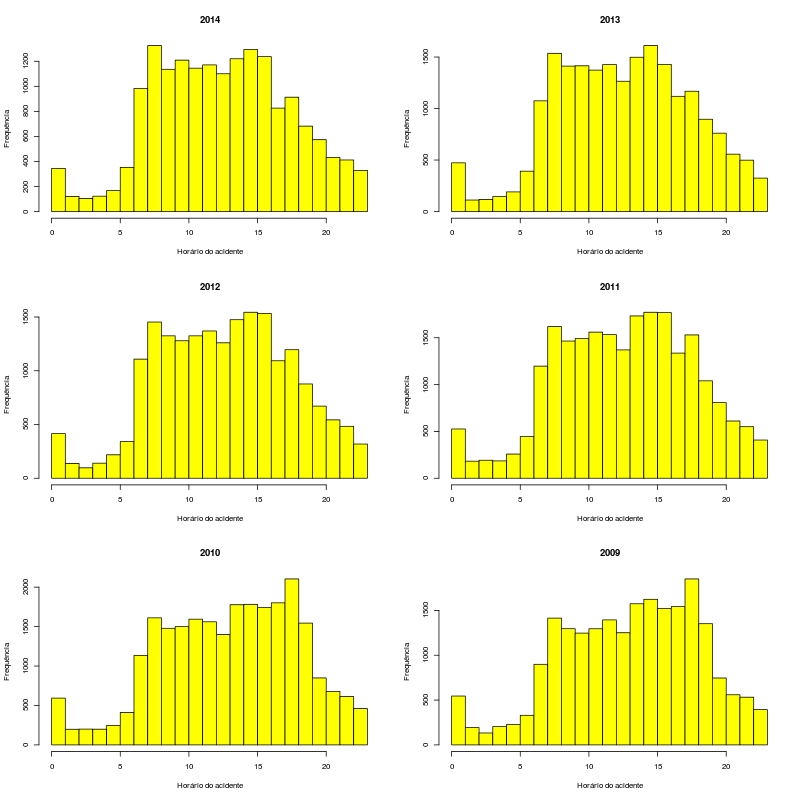
\includegraphics[width=\textwidth]{horas_acidentes.jpg}
\end{figure}

Na observação individual dos histogramas nota-se um comportamento de que os acidentes ocorriam entre 16 e 18 horas, sendo que, nos últimos anos este comportamento se modificou e os acidentes começaram a ter uma maior densidade entre as 13 e 15 horas, sendo que o período das 7 até as 16 horas é o período de maiores ocorrências. Os acidentes no período de 2014 tiveram um leve aumento após as 15 horas em relação aos anos anteriores, sendo que o período das manhã teve um leve aumento na densidade de acidentes.

\begin{figure}[h!]
	\caption{Histogramas dos meses dos acidentes entre 2009 e 2014} \label{fig:histmes}
    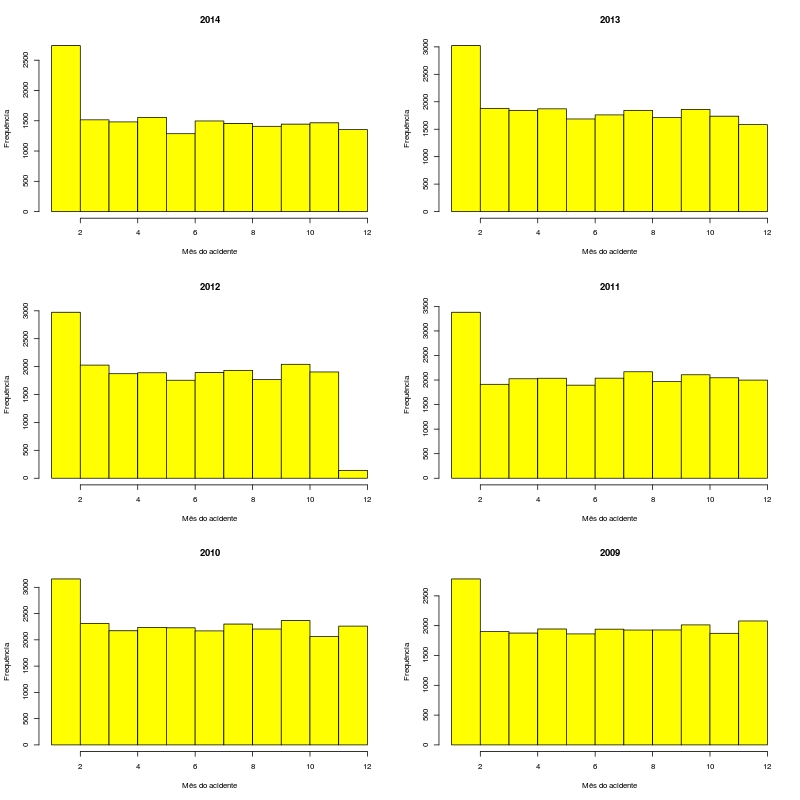
\includegraphics[width=\textwidth]{meses_acidentes.jpg}
\end{figure}

Nos meses de acidentes, conforme observado na Figura \ref{fig:histmes} apenas o período de Janeiro teve um aumento significativo em todos os anos, o que provavelmente está relacionado com as férias escolares e com a chegada da temporada de verão, sendo que Porto Alegre tem várias conexões, principalmente para estradas que tem um grande fluxo e que leva ao litoral, como a FreeWay.

Depois de uma análise do profile dos dados, tentou-se explicar se há alguma influência no tipo de veículo utilizado em relação aos acidentes, então, a \textbf{correlação} foi aplicada para tentar explicar se existe alguma influência, conforme pode ser visto na Tabela \ref{tab:corr}. Caso houvesse correlação com o tipo de veículo, poderia ser feito ações para estes veículos especificadamente.

\begin{table}[ht]
\centering
\begin{small}
\caption{Correlação entre acidentes fatais e tipo de veículo} \label{tab:corr}
\begin{tabular}{l|r|r|r|r|r|r|r|r|r|r}
  \hline
\multicolumn{1}{c|}{\textbf{Tipo}} & \multicolumn{1}{c|}{\textbf{Auto}} & \multicolumn{1}{c|}{\textbf{Taxi}} & \multicolumn{1}{c|}{\textbf{Lot.}} & \multicolumn{1}{c|}{\textbf{O.U.}} & \multicolumn{1}{c|}{\textbf{O.I.}} & \multicolumn{1}{c|}{\textbf{Cam.}} & \multicolumn{1}{c|}{\textbf{Mot.}} & \multicolumn{1}{c|}{\textbf{Car.}} & \multicolumn{1}{c|}{\textbf{Bic.}} & \multicolumn{1}{c}{\textbf{Out.}} \\ \hline
FATAIS & 0.09 & -0.02 & -0.01 & -0.01 & 0.02 & -0.02 & -0.03 & -0.01 & -0.04 & -0.01 \\ 
\# $\dagger$ & 0.01 & -0.04 & 0.03 & 0.03 & 0.04 & 0.09 & 0.04 & 0.03 & -0.06 & 0.03 \\ 
\# $\dagger$ pos.& 0.03 & 0.03 & -0.04 & -0.04 & -0.04 & -0.11 & -0.06 & -0.04 & 0.04 & -0.04 \\ 
   \hline
\end{tabular}
\end{small}
\end{table}

Apresentaram-se as correlações fracas para todos os tipos de veículos, portanto, não há influência de acidentes do tipo fatal em relação a algum tipo específico de veículo, descartando a hipótese de ter, por exemplo, uma relação gritante de acidentes de motos serem os mais fatais. 

Neste ponto vale criticar que não temos a informação de qual veículo teve relação com vítimas fatais. Por exemplo, se o acidente envolveu um carro e uma moto, na correlação não temos como identificar qual era o veículo que no momento do acidente acarretou na morte da vítima, portanto, considera-se que a informação não seria suficiente para inferir mais detalhes sobre o tipo de veículo envolvido no acidente e a relação direta com a vítima.

Em relação ao algoritmo \textbf{\textit{apriori}}, para acidentes fatais os resultados não obtiveram valores significantes sendo que para inferir alguma informação o suporte e a confidência tinham valores extremamente baixos como suporte=$0.01$ e confidência=$0.2$, portanto, o algoritmo \textit{apriori} para detecção de padrões em acidentes do tipo fatais não tiveram uma boa resposta ou uma boa calibragem, neste caso nenhuma inferência pode ser feita a partir deste algoritmo.

Para analisar então quais são os fatores dos acidentes fatais, criou-se dataset auxiliar (detalhado no pré-processamento) somente com acidentes do tipo fatais e com as seguintes colunas: NOITE\_DIA, LOCAL, LOG1, TIPO\_ACID, DIA\_SEM, TEMPO, REGIAO. As colunas escolhidas foram as que naturalmente eram fatores. 

Nas rodadas, o algoritmo \textit{apriori} foi rodado várias vezes com várias configurações e os resultados com suporte em=$0.1$ e confiança=$0.8$ obteve-se alguns dados interessantes, sendo:

\begin{itemize}
	\item Os acidentes fatais do tipo atropelamento tem uma predominância de acontecer no centro da cidade, durante o dia e com tempo bom. 
	\item Os acidentes que ocorrem à noite estão relacionados mais a um local, a Avenida Baltazar de Oliveira Garcia.
	\item Os choques tem uma forte relação com o dia de sábado.
	\item Os atropelamentos ocorrem principalmente na Cristóvão Colombo e na Farrapos
	\item Os acidentes em cruzamentos tem forte relação com o turno da noite
\end{itemize}

Para tentar identificar características de acidentes fatais e não-fatais o algoritmo k-nn foi executado. Inicialmente, um \textit{dataset} com campos específicos foi criado, contando com os campos CAMPOS, após isso, os resultados da execução trouxeram as seguintes informações.

Por último, a criação de um \textit{"heatmap"}\ interativo com a densidade de acidentes foi criado de forma a ter uma visualização dos acidentes ano a ano e pelo período completo para permitir analisar os locais que são mais críticos em relação a acidentes, tanto fatais quanto não fatais.

\begin{figure}[h!]
	\caption{Densidades de acidentes fatais de 2009 até 2014 com pardais e lombadas} \label{fig:densaci0914}
	\centering
	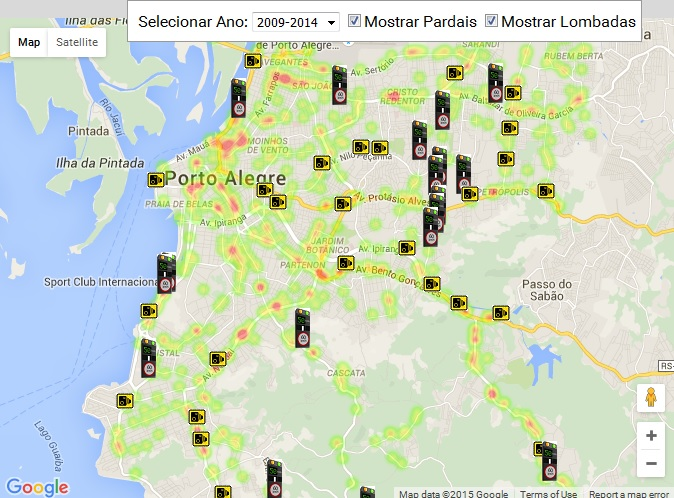
\includegraphics[width=.8\textwidth]{densidade_acidentes_2009_a_2014.jpg}
\end{figure}

\begin{figure}[h!]
	\caption{Densidades de acidentes fatais em 2014 com pardais e lombadas} \label{fig:densaci}
	\centering
	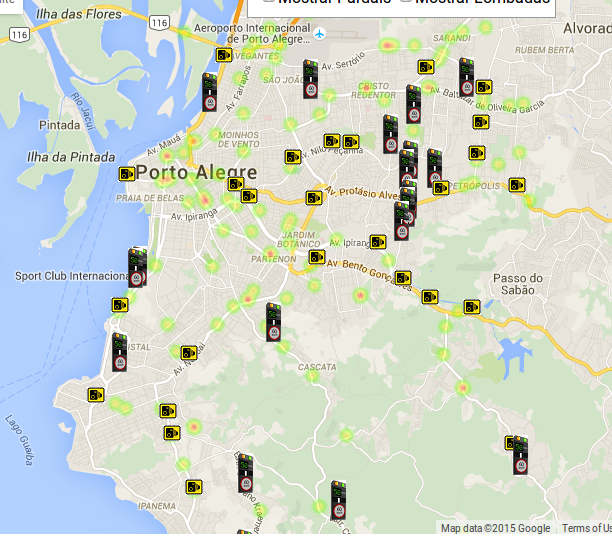
\includegraphics[width=.8\textwidth]{densidade_acidentes_2014.jpg}
\end{figure}

A geração de mapa com densidades dos acidentes foi feita utilizando-se dos dados de latitude e longitude dos acidentes, classificando os seguintes tipos de acidentes: fatais, com feridos graves, com feridos e todos. O local da latitude e longitude foi marcado conforme a densidade de acidentes no local. 

Também, neste momento foi utilizado os outros dois datasets disponíveis, os datasets de localização de pardais e o de localização de lombadas eletrônicas sendo marcados pela latitude e longitude pré-processada. 

O resultado nos traz um mapa interativo demonstrando as densidades dos acidentes relacionados de 2009 a 2014, conforme ilustrado na Figura \ref{fig:densaci0914}, e também ano a ano, conforme ilustrado na Figura \ref{fig:densaci}, pontos verdes indicam acidentes fatais, quanto mais perto da cor vermelha os pontos, maior a densidade de acidentes fatais no local.

Para o mapa com densidades houve a necessidade de programação com a API do Google Maps para permitir uma interatividade com os dados.

Os resultados obtidos com o \textit{dataset} permitiu verificar que os acidentes ocorrem logo após as curvas, também, os acidentes acontecem antes e depois da localização das lombadas eletrônicas, porém, não ocorrem acidentes no local da lombada. Alguns pontos mais críticos foram localizados pela visualização da densidade, como locais no centro e em alguns cruzamentos de avenidas.

A seguir (seção \ref{sec:conclusao}) apresentamos as conclusões da análise dos datasets, buscando um ponto de vista mais de gestão bem como considerações finais do trabalho.


\section{Conclusões}
\label{sec:conclusao}

Primeiramente, a análise dos dados permitiu uma compreensão melhor do comportamento dos acidentes na cidade de Porto Alegre, fazendo com que trouxesse informações interessantes assim, com as informações evidenciadas, ações poderiam envolver uma melhoria no trânsito.

Na parte de pré-processamento, mesmo sendo uma base de dados padronizada e voltada para a utilização como dataset, os dados fornecidos tinham algumas inconsistências ao qual tiveram um custo até o seu conhecimento e ajuste da informação bem como, diferenças entre os arquivos, ao qual, não estão explícitos no fornecimento da informação. Também, o pré-processamento permitiu a união da informação por meio da padronização das informações, como, por exemplo, utilização de tipos e dados específicos para certas técnicas, como o algoritmo \textit{apriori}.

Os histogramas e o \textit{profiling} dos dados mostrou alguns comportamentos padrões entre os anos analisados, demonstrando uma diminuição no número de acidentes, porém, um aumento em relação ao número de acidentes fatais.

As correlações, ao qual tentava-se identificar alguma relação entre acidente fatal e tipo de veículo não demonstrou relevâncias suficientes, portanto, não há influência no tipo de transporte em relação a acidentes fatais, feridos ou feridos graves.

Também, o mapa com a densidade dos acidentes comprovou que locais com controladores de velocidade e pardais os acidentes fatais são bem raros, mostrando-se um sistema eficiente para diminuição dos acidentes. Outro ponto importante que pode ser visto no mapa são os locais com maiores quantidades de acidentes. 

Também notou-se que os acidentes mais graves ocorrem em entradas de vias principais, como, por exemplo, a Av. Bento Gonçalves. Nas próprias avenidas não há registros de acidentes graves, porém, logo após as entradas secundárias destas avenidas pode-se verificar registros com densidades consideráveis de serem avaliadas.

Também, notou-se que durante a madrugada a incidência de acidentes do tipo fatal é menor em relação ao período do dia por, justamente ter menos fluxo de carros que durante o dia. 

Pelo algoritmo \textit{apriori} pode-se constatar que existe um local de acidentes fatais à noite, a Av. Baltazar de Oliveira, para este local sugere-se um estudo para diminuir os acidentes, seja sinalizando, mudando rotas ou apenas melhorando sua iluminação. 

Foi possível inferir que no centro da cidade é onde há a maior incidência de atropelamentos fatais, para tanto, campanhas de conscientização deveriam ser feitas para amenizar o problema bem como o aumento da fiscalização.

Como sugestões de melhoria no trânsito, temos:

\begin{itemize}
	\item[-] Melhorar sinalização nas esquinas, principalmente nas vias de entrada das principais avenidas por conterem o maior número de acidentes do tipo fatais
	\item[-] Em vias com um grande número de acidentes fatais diminuir a velocidade máxima ou realizar blitz, como, por exemplo, a Estrada João de Oliveira Remião.
	\item[-] Aumentar a sinalização onde as densidades dos acidentes ocorrem mais
	\item[-] Refazer o KDD anualmente, na medida que as informações dos datasets estão disponíveis para verificar o comportamento do trânsito e inferir novas ações;
\end{itemize}

Por fim, o presente trabalho trouxe para os autores uma boa experiência em relação ao que pode ser feito com uma estrutura de dados, várias inferências a partir de um conjunto de dados pode ser feita bem como, pela junção de informações que corroboram (como no caso das lombadas e pardais) em relação aos dados disponíveis.

Como sugestão de trabalhos futuros, recomenda-se estudar outros datasets disponíveis em relação ao trânsito de Porto Alegre, como a base de operações e apreensões em \textit{blitz} de forma a enriquecer as análises com maiores informações. 

\newpage
\section*{ANEXOS}
ANEXO I - CÓDIGO R UTILIZADO NA ANÁLISE DOS DADOS

\begin{small}
\begin{lstlisting}[language=R,frame=shadowbox, breaklines=true, commentstyle=\textit]

acidentes2009 <- read.csv("acidentes-2009.csv", header=TRUE, sep=";")
acidentes2010 <- read.csv("acidentes-2010.csv", header=TRUE, sep=";")
acidentes2011 <- read.csv("acidentes-2011.csv", header=TRUE, sep=";")
acidentes2012 <- read.csv("acidentes-2012.csv", header=TRUE, sep=";")
acidentes2013 <- read.csv("acidentes-2013.csv", header=TRUE, sep=";")
acidentes2014 <- read.csv("acidentes-2014.csv", header=TRUE, sep=";")

# Contando numero de acidentes
length(acidentes2009)
length(acidentes2010)
length(acidentes2011)
length(acidentes2012)
length(acidentes2013)
length(acidentes2014)

# Verificando acidentes fatais
summary(as.factor(acidentes2009$FATAIS))
summary(as.factor(acidentes2010$FATAIS))
summary(as.factor(acidentes2011$FATAIS))
summary(as.factor(acidentes2012$FATAIS))
summary(as.factor(acidentes2013$FATAIS))
summary(as.factor(acidentes2014$FATAIS))

# Somando numero de mortes
sum(acidentes2009$MORTE_POST)+sum(acidentes2009$MORTES)
sum(acidentes2010$MORTE_POST)+sum(acidentes2010$MORTES)
sum(acidentes2011$MORTE_POST)+sum(acidentes2011$MORTES)
sum(acidentes2012$MORTE_POST)+sum(acidentes2012$MORTES)
sum(acidentes2013$MORTE_POST)+sum(acidentes2013$MORTES)
sum(acidentes2014$MORTE_POST)+sum(acidentes2014$MORTES)

# Desconsiderando valores vazios
na.rm=T

# Verificando valores minimos e maximos
range(acidentes2009$MORTE_POST)
range(acidentes2010$MORTE_POST)
range(acidentes2011$MORTE_POST)
range(acidentes2012$MORTE_POST)
range(acidentes2013$MORTE_POST)
range(acidentes2014$MORTE_POST)

range(acidentes2009$MORTES)
range(acidentes2010$MORTES)
range(acidentes2011$MORTES)
range(acidentes2012$MORTES)
range(acidentes2013$MORTES)
range(acidentes2014$MORTES)

range(acidentes2009$FATAIS)
range(acidentes2010$FATAIS)
range(acidentes2011$FATAIS)
range(acidentes2012$FATAIS)
range(acidentes2013$FATAIS)
range(acidentes2014$FATAIS)

length(which(as.numeric(acidentes2009$FATAIS)>=1))
length(which(as.numeric(acidentes2010$FATAIS)>=1))
length(which(as.numeric(acidentes2011$FATAIS)>=1))
length(which(as.numeric(acidentes2012$FATAIS)>=1))
length(which(as.numeric(acidentes2013$FATAIS)>=1))
length(which(as.numeric(acidentes2014$FATAIS)>=1))

# Gerando histogramas de horarios de acidentes

jpeg(filename="horas_acidentes.jpg", width=800, height=800, units="px", pointsize=12, quality=100, bg="white", res=NA);
par(mfrow=c(3,2))
hist(as.numeric(acidentes2014$FX_HORA), breaks=24, main="2014", xlab="Horario do acidente", ylab="Frequencia", col="yellow");
hist(as.numeric(acidentes2013$FX_HORA), breaks=24, main="2013", xlab="Horario do acidente", ylab="Frequencia", col="yellow");
hist(as.numeric(acidentes2012$FX_HORA), breaks=24, main="2012", xlab="Horario do acidente", ylab="Frequencia", col="yellow");
hist(as.numeric(acidentes2011$FX_HORA), breaks=24, main="2011", xlab="Horario do acidente", ylab="Frequencia", col="yellow");
hist(as.numeric(acidentes2010$FX_HORA), breaks=24, main="2010", xlab="Horario do acidente", ylab="Frequencia", col="yellow");
hist(as.numeric(acidentes2009$FX_HORA), breaks=24, main="2009", xlab="Horario do acidente", ylab="Frequencia", col="yellow");
dev.off()

jpeg(filename="meses_acidentes.jpg", width=800, height=800, units="px", pointsize=12, quality=100, bg="white", res=NA);
par(mfrow=c(3,2))
hist(as.numeric(acidentes2014$MES), breaks=12, main="2014", xlab="Mes do acidente", ylab="Frequencia", col="yellow");
hist(as.numeric(acidentes2013$MES), breaks=12, main="2013", xlab="Mes do acidente", ylab="Frequencia", col="yellow");
hist(as.numeric(acidentes2012$MES), breaks=12, main="2012", xlab="Mes do acidente", ylab="Frequencia", col="yellow");
hist(as.numeric(acidentes2011$MES), breaks=12, main="2011", xlab="Mes do acidente", ylab="Frequencia", col="yellow");
hist(as.numeric(acidentes2010$MES), breaks=12, main="2010", xlab="Mes do acidente", ylab="Frequencia", col="yellow");
hist(as.numeric(acidentes2009$MES), breaks=12, main="2009", xlab="Mes do acidente", ylab="Frequencia", col="yellow");
dev.off()

fatais2014 <- data.frame(cbind(AUTO = subset(acidentes2014, FATAIS != 0)$AUTO, TAXI = subset(acidentes2014, FATAIS != 0)$TAXI, LOTACAO = subset(acidentes2014, FATAIS != 0)$LOTACAO, ONIBUS_URB = subset(acidentes2014, FATAIS != 0)$ONIBUS_URB, ONIBUS_INT = subset(acidentes2014, FATAIS != 0)$ONIBUS_INT, CAMINHAO = subset(acidentes2014, FATAIS != 0)$CAMINHAO, MOTO = subset(acidentes2014, FATAIS != 0)$MOTO, CARROCA = subset(acidentes2014, FATAIS != 0)$CARROCA, BICICLETA = subset(acidentes2014, FATAIS != 0)$BICICLETA, OUTRO = subset(acidentes2014, FATAIS != 0)$OUTRO, FATAIS = subset(acidentes2014, FATAIS != 0)$FATAIS, MORTES = subset(acidentes2014, FATAIS != 0)$MORTES, MORTE_POST = subset(acidentes2014, FATAIS != 0)$MORTE_POST, FERIDOS = subset(acidentes2014, FATAIS != 0)$FERIDOS))

fatais2013 <- data.frame(cbind(AUTO = subset(acidentes2013, FATAIS != 0)$AUTO, TAXI = subset(acidentes2013, FATAIS != 0)$TAXI, LOTACAO = subset(acidentes2013, FATAIS != 0)$LOTACAO, ONIBUS_URB = subset(acidentes2013, FATAIS != 0)$ONIBUS_URB, ONIBUS_INT = subset(acidentes2013, FATAIS != 0)$ONIBUS_INT, CAMINHAO = subset(acidentes2013, FATAIS != 0)$CAMINHAO, MOTO = subset(acidentes2013, FATAIS != 0)$MOTO, CARROCA = subset(acidentes2013, FATAIS != 0)$CARROCA, BICICLETA = subset(acidentes2013, FATAIS != 0)$BICICLETA, OUTRO = subset(acidentes2013, FATAIS != 0)$OUTRO, FATAIS = subset(acidentes2013, FATAIS != 0)$FATAIS, MORTES = subset(acidentes2013, FATAIS != 0)$MORTES, MORTE_POST = subset(acidentes2013, FATAIS != 0)$MORTE_POST, FERIDOS = subset(acidentes2013, FATAIS != 0)$FERIDOS))

fatais2012 <- data.frame(cbind(AUTO = subset(acidentes2012, FATAIS != 0)$AUTO, TAXI = subset(acidentes2012, FATAIS != 0)$TAXI, LOTACAO = subset(acidentes2012, FATAIS != 0)$LOTACAO, ONIBUS_URB = subset(acidentes2012, FATAIS != 0)$ONIBUS_URB, ONIBUS_INT = subset(acidentes2012, FATAIS != 0)$ONIBUS_INT, CAMINHAO = subset(acidentes2012, FATAIS != 0)$CAMINHAO, MOTO = subset(acidentes2012, FATAIS != 0)$MOTO, CARROCA = subset(acidentes2012, FATAIS != 0)$CARROCA, BICICLETA = subset(acidentes2012, FATAIS != 0)$BICICLETA, OUTRO = subset(acidentes2012, FATAIS != 0)$OUTRO, FATAIS = subset(acidentes2012, FATAIS != 0)$FATAIS, MORTES = subset(acidentes2012, FATAIS != 0)$MORTES, MORTE_POST = subset(acidentes2012, FATAIS != 0)$MORTE_POST, FERIDOS = subset(acidentes2012, FATAIS != 0)$FERIDOS))

fatais2011 <- data.frame(cbind(AUTO = subset(acidentes2011, FATAIS != 0)$AUTO, TAXI = subset(acidentes2011, FATAIS != 0)$TAXI, LOTACAO = subset(acidentes2011, FATAIS != 0)$LOTACAO, ONIBUS_URB = subset(acidentes2011, FATAIS != 0)$ONIBUS_URB, ONIBUS_INT = subset(acidentes2011, FATAIS != 0)$ONIBUS_INT, CAMINHAO = subset(acidentes2011, FATAIS != 0)$CAMINHAO, MOTO = subset(acidentes2011, FATAIS != 0)$MOTO, CARROCA = subset(acidentes2011, FATAIS != 0)$CARROCA, BICICLETA = subset(acidentes2011, FATAIS != 0)$BICICLETA, OUTRO = subset(acidentes2011, FATAIS != 0)$OUTRO, FATAIS = subset(acidentes2011, FATAIS != 0)$FATAIS, MORTES = subset(acidentes2011, FATAIS != 0)$MORTES, MORTE_POST = subset(acidentes2011, FATAIS != 0)$MORTE_POST, FERIDOS = subset(acidentes2011, FATAIS != 0)$FERIDOS))

fatais2010 <- data.frame(cbind(AUTO = subset(acidentes2010, FATAIS != 0)$AUTO, TAXI = subset(acidentes2010, FATAIS != 0)$TAXI, LOTACAO = subset(acidentes2010, FATAIS != 0)$LOTACAO, ONIBUS_URB = subset(acidentes2010, FATAIS != 0)$ONIBUS_URB, ONIBUS_INT = subset(acidentes2010, FATAIS != 0)$ONIBUS_INT, CAMINHAO = subset(acidentes2010, FATAIS != 0)$CAMINHAO, MOTO = subset(acidentes2010, FATAIS != 0)$MOTO, CARROCA = subset(acidentes2010, FATAIS != 0)$CARROCA, BICICLETA = subset(acidentes2010, FATAIS != 0)$BICICLETA, OUTRO = subset(acidentes2010, FATAIS != 0)$OUTRO, FATAIS = subset(acidentes2010, FATAIS != 0)$FATAIS, MORTES = subset(acidentes2010, FATAIS != 0)$MORTES, MORTE_POST = subset(acidentes2010, FATAIS != 0)$MORTE_POST, FERIDOS = subset(acidentes2010, FATAIS != 0)$FERIDOS))

fatais2009 <- data.frame(cbind(AUTO = subset(acidentes2009, FATAIS != 0)$AUTO, TAXI = subset(acidentes2009, FATAIS != 0)$TAXI, LOTACAO = subset(acidentes2009, FATAIS != 0)$LOTACAO, ONIBUS_URB = subset(acidentes2009, FATAIS != 0)$ONIBUS_URB, ONIBUS_INT = subset(acidentes2009, FATAIS != 0)$ONIBUS_INT, CAMINHAO = subset(acidentes2009, FATAIS != 0)$CAMINHAO, MOTO = subset(acidentes2009, FATAIS != 0)$MOTO, CARROCA = subset(acidentes2009, FATAIS != 0)$CARROCA, BICICLETA = subset(acidentes2009, FATAIS != 0)$BICICLETA, OUTRO = subset(acidentes2009, FATAIS != 0)$OUTRO, FATAIS = subset(acidentes2009, FATAIS != 0)$FATAIS, MORTES = subset(acidentes2009, FATAIS != 0)$MORTES, MORTE_POST = subset(acidentes2009, FATAIS != 0)$MORTE_POST, FERIDOS = subset(acidentes2009, FATAIS != 0)$FERIDOS))


fatais <- rbind(fatais2014, fatais2013)
fatais <- rbind(fatais, fatais2012)
fatais <- rbind(fatais, fatais2011)
fatais <- rbind(fatais, fatais2010)
fatais <- rbind(fatais, fatais2009)

# Correlacoes
correlacoes = data.frame(rbind( 
  FATAIS = c(AUTO = cor(fatais$FATAIS, fatais$AUTO), TAXI = cor(fatais$FATAIS, fatais$TAXI),LOACAO = cor(fatais$FATAIS, fatais$LOTACAO),ONIBUS_URB = cor(fatais$FATAIS, fatais$ONIBUS_URB),ONIBUS_INT = cor(fatais$FATAIS, fatais$ONIBUS_INT),CAMINHAO = cor(fatais$FATAIS, fatais$CAMINHAO), MOTO = cor(fatais$FATAIS, fatais$MOTO),CARROCA = cor(fatais$FATAIS, fatais$CARROCA), BICICLETA = cor(fatais$FATAIS, fatais$BICICLETA), OUTRO = cor(fatais$FATAIS, fatais$OUTRO)), 
  MORTES = c(cor(fatais$MORTES, fatais$AUTO), cor(fatais$MORTES, fatais$TAXI), cor(fatais$MORTES, fatais$LOTACAO), cor(fatais$MORTES, fatais$ONIBUS_URB), cor(fatais$MORTES, fatais$ONIBUS_INT), cor(fatais$MORTES, fatais$CAMINHAO), cor(fatais$MORTES, fatais$MOTO), cor(fatais$MORTES, fatais$CARROCA), cor(fatais$MORTES, fatais$BICICLETA), cor(fatais$MORTES, fatais$OUTRO)), 
  MORTES_POST = c(cor(fatais$MORTE_POST, fatais$AUTO), cor(fatais$MORTE_POST, fatais$TAXI), cor(fatais$MORTE_POST, fatais$LOTACAO), cor(fatais$MORTE_POST, fatais$ONIBUS_URB), cor(fatais$MORTE_POST, fatais$ONIBUS_INT), cor(fatais$MORTE_POST, fatais$CAMINHAO), cor(fatais$MORTE_POST, fatais$MOTO), cor(fatais$MORTE_POST, fatais$CARROCA), cor(fatais$MORTE_POST, fatais$BICICLETA), cor(fatais$MORTE_POST, fatais$OUTRO)), 
  FERIDOS = c(cor(fatais$FERIDOS, fatais$AUTO), cor(fatais$FERIDOS, fatais$TAXI), cor(fatais$FERIDOS, fatais$LOTACAO), cor(fatais$FERIDOS, fatais$ONIBUS_URB), cor(fatais$FERIDOS, fatais$ONIBUS_INT), cor(fatais$FERIDOS, fatais$CAMINHAO), cor(fatais$FERIDOS, fatais$MOTO), cor(fatais$FERIDOS, fatais$CARROCA), cor(fatais$FERIDOS, fatais$BICICLETA), cor(fatais$FERIDOS, fatais$OUTRO))))

#
# APRIORI
#
fatais2014 <- data.frame(NOITEDIA = subset(acidentes2014, FATAIS != 0)$NOITE_DIA, LOCAL = subset(acidentes2014, FATAIS != 0)$LOCAL, DIASEM = subset(acidentes2014, FATAIS != 0)$DIA_SEM, LOG1 = subset(acidentes2014, FATAIS != 0)$LOG1, TIPO_ACID = subset(acidentes2014, FATAIS != 0)$TIPO_ACID, LOCAL = subset(acidentes2014, FATAIS != 0)$LOCAL, TEMPO = subset(acidentes2014, FATAIS != 0)$TEMPO, REGIAO = subset(acidentes2014, FATAIS != 0)$REGIAO)

fatais2013 <- data.frame(NOITEDIA = subset(acidentes2013, FATAIS != 0)$NOITE_DIA, LOCAL = subset(acidentes2013, FATAIS != 0)$LOCAL, DIASEM = subset(acidentes2013, FATAIS != 0)$DIA_SEM, LOG1 = subset(acidentes2013, FATAIS != 0)$LOG1, TIPO_ACID = subset(acidentes2013, FATAIS != 0)$TIPO_ACID, LOCAL = subset(acidentes2013, FATAIS != 0)$LOCAL, TEMPO = subset(acidentes2013, FATAIS != 0)$TEMPO, REGIAO = subset(acidentes2013, FATAIS != 0)$REGIAO)

fatais2012 <- data.frame(NOITEDIA = subset(acidentes2012, FATAIS != 0)$NOITE_DIA, LOCAL = subset(acidentes2012, FATAIS != 0)$LOCAL, DIASEM = subset(acidentes2012, FATAIS != 0)$DIA_SEM, LOG1 = subset(acidentes2012, FATAIS != 0)$LOG1, TIPO_ACID = subset(acidentes2012, FATAIS != 0)$TIPO_ACID, LOCAL = subset(acidentes2012, FATAIS != 0)$LOCAL, TEMPO = subset(acidentes2012, FATAIS != 0)$TEMPO, REGIAO = subset(acidentes2012, FATAIS != 0)$REGIAO)

fatais2011 <- data.frame(NOITEDIA = subset(acidentes2011, FATAIS != 0)$NOITE_DIA, LOCAL = subset(acidentes2011, FATAIS != 0)$LOCAL, DIASEM = subset(acidentes2011, FATAIS != 0)$DIA_SEM, LOG1 = subset(acidentes2011, FATAIS != 0)$LOG1, TIPO_ACID = subset(acidentes2011, FATAIS != 0)$TIPO_ACID, LOCAL = subset(acidentes2011, FATAIS != 0)$LOCAL, TEMPO = subset(acidentes2011, FATAIS != 0)$TEMPO, REGIAO = subset(acidentes2011, FATAIS != 0)$REGIAO)

fatais2010 <- data.frame(NOITEDIA = subset(acidentes2010, FATAIS != 0)$NOITE_DIA, LOCAL = subset(acidentes2010, FATAIS != 0)$LOCAL, DIASEM = subset(acidentes2010, FATAIS != 0)$DIA_SEM, LOG1 = subset(acidentes2010, FATAIS != 0)$LOG1, TIPO_ACID = subset(acidentes2010, FATAIS != 0)$TIPO_ACID, LOCAL = subset(acidentes2010, FATAIS != 0)$LOCAL, TEMPO = subset(acidentes2010, FATAIS != 0)$TEMPO, REGIAO = subset(acidentes2010, FATAIS != 0)$REGIAO)

fatais2009 <- data.frame(NOITEDIA = subset(acidentes2009, FATAIS != 0)$NOITE_DIA, LOCAL = subset(acidentes2009, FATAIS != 0)$LOCAL, DIASEM = subset(acidentes2009, FATAIS != 0)$DIA_SEM, LOG1 = subset(acidentes2009, FATAIS != 0)$LOG1, TIPO_ACID = subset(acidentes2009, FATAIS != 0)$TIPO_ACID, LOCAL = subset(acidentes2009, FATAIS != 0)$LOCAL, TEMPO = subset(acidentes2009, FATAIS != 0)$TEMPO, REGIAO = subset(acidentes2009, FATAIS != 0)$REGIAO)

fatais <- merge(fatais2014, fatais2013, all=TRUE)
fatais <- merge(fatais, fatais2012, all=TRUE)
fatais <- merge(fatais, fatais2011, all=TRUE)
fatais <- merge(fatais, fatais2010, all=TRUE)
fatais <- merge(fatais, fatais2009, all=TRUE)

library(arules)
rules <- apriori(fatais, parameter = list(minlen=2, sup=0.005, conf=0.8), appearance = list(rhs=c("NOITEDIA=NOITE","NOITEDIA=DIA"), default="lhs"), control=list(verbose=F))
inspect(rules)
rules <- apriori(fatais, parameter = list(minlen=2, sup=0.01, conf=0.8), appearance = list(rhs=c("TIPO_ACID=ATROPELAMENTO", "TIPO_ACID=CHOQUE", "TIPO_ACID=ALBAROAMENTO"), default="lhs"), control=list(verbose=F))
inspect(rules)
\end{lstlisting}
\end{small}

\end{document}